\begin{LARGE}
  \textbf{Part 2: New project below}
\end{LARGE}

\hspace*{\fill}

You are secret agent Melbourne Wrist-toe, a member of the top-secret SD-320 organization. Your friends all believe your cover story – that you are a UMassD ECE student. Working with your partner Mason, you acquired one of the coveted Ravioli manuscripts drawn by the 15th century genius and architect Manicotti Ravioli. This particular manuscript includes a diagram for a speech scrambling system, shown below in Figure 1, which was used to encode a secret message from Ravioli. Some of the important parts of the diagram in the Ravioli manuscript were damaged when you recovered it from your rival organization, ejω -Directorate. Working with the SD-320 technology guru Fender, you need to use the diagram from the manuscript to write a Matlab program that will unscramble the speech and recover the secret message.


\begin{figure}[!htbp]
  \centering
    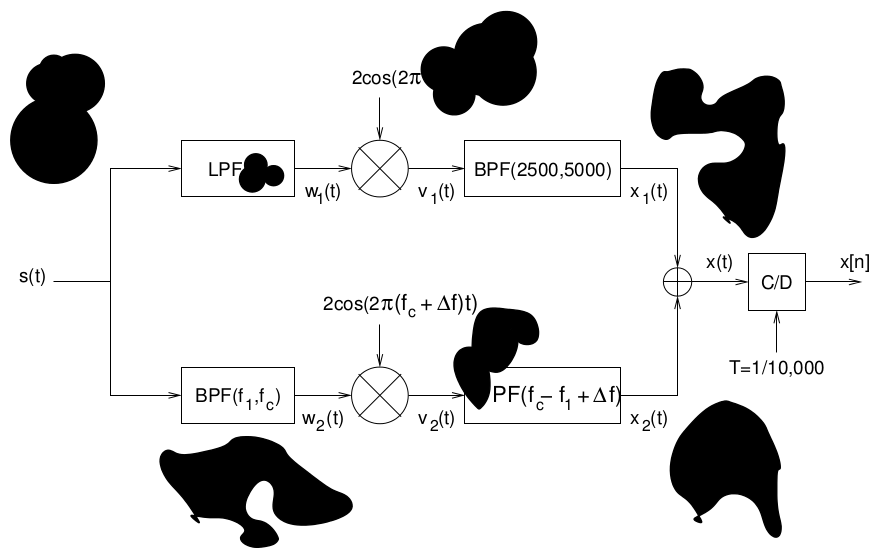
\includegraphics[width=0.7\textwidth]{Part2/Question/Ravioli.png}
  \caption{Secret speech scrambler from the Ravioli manuscript}
\end{figure}

